% Preamble
\documentclass[11pt]{article}

% Packages
\usepackage[spanish]{babel}
\usepackage[margin=2.54cm]{geometry}
\usepackage{amsmath}
\usepackage{amsfonts}
\usepackage{xcolor}
\usepackage{float}
\usepackage{graphicx}
\usepackage{listings}
% Title
\title{EVALUACIÓN FINAL - SOLUCIÓN}
\author{Jhon Roly Ordoñez Leon}
\date{\today}

% Program code
\definecolor{codegreen}{rgb}{0,0.6,0}
\definecolor{codegray}{rgb}{0.5,0.5,0.5}
\definecolor{codepurple}{rgb}{0.58,0,0.82}
\definecolor{backcolour}{rgb}{0.95,0.95,0.92}
\lstdefinestyle{mystyle}{
	backgroundcolor=\color{backcolour},   
	commentstyle=\color{codegreen},
	keywordstyle=\color{magenta},
	numberstyle=\tiny\color{codegray},
	stringstyle=\color{codepurple},
	identifierstyle=\color{blue},
	basicstyle=\ttfamily\footnotesize,
	breakatwhitespace=false,         
	breaklines=true,                 
	captionpos=b,                    
	keepspaces=true,
	numbers=left,                    
	numbersep=5pt,                  
	showspaces=false,                
	showstringspaces=false,
	showtabs=false,                  
	tabsize=2
}
\lstset{style=mystyle}



% Document
\begin{document}
	\maketitle
	
	% Pregunta 1
	\section*{Elija un giro de negocio}
	
	EL giro de negocio que elijo de las tres alternativas(Mecánica de autos, Biblioteca y Clínica) que se tiene  para la solución de esta evaluación es \textcolor{blue}{Biblioteca} 
	
	% Pregunta 2
	\section*{Cree un DER que muestre la relación entre 3 entidades. 2 ptos}
	
	A continuación se muestra el Diagrama Entidad Relación (DER) creado usando el yEd Graph Editor.
		\begin{figure}[H]
			\centering
			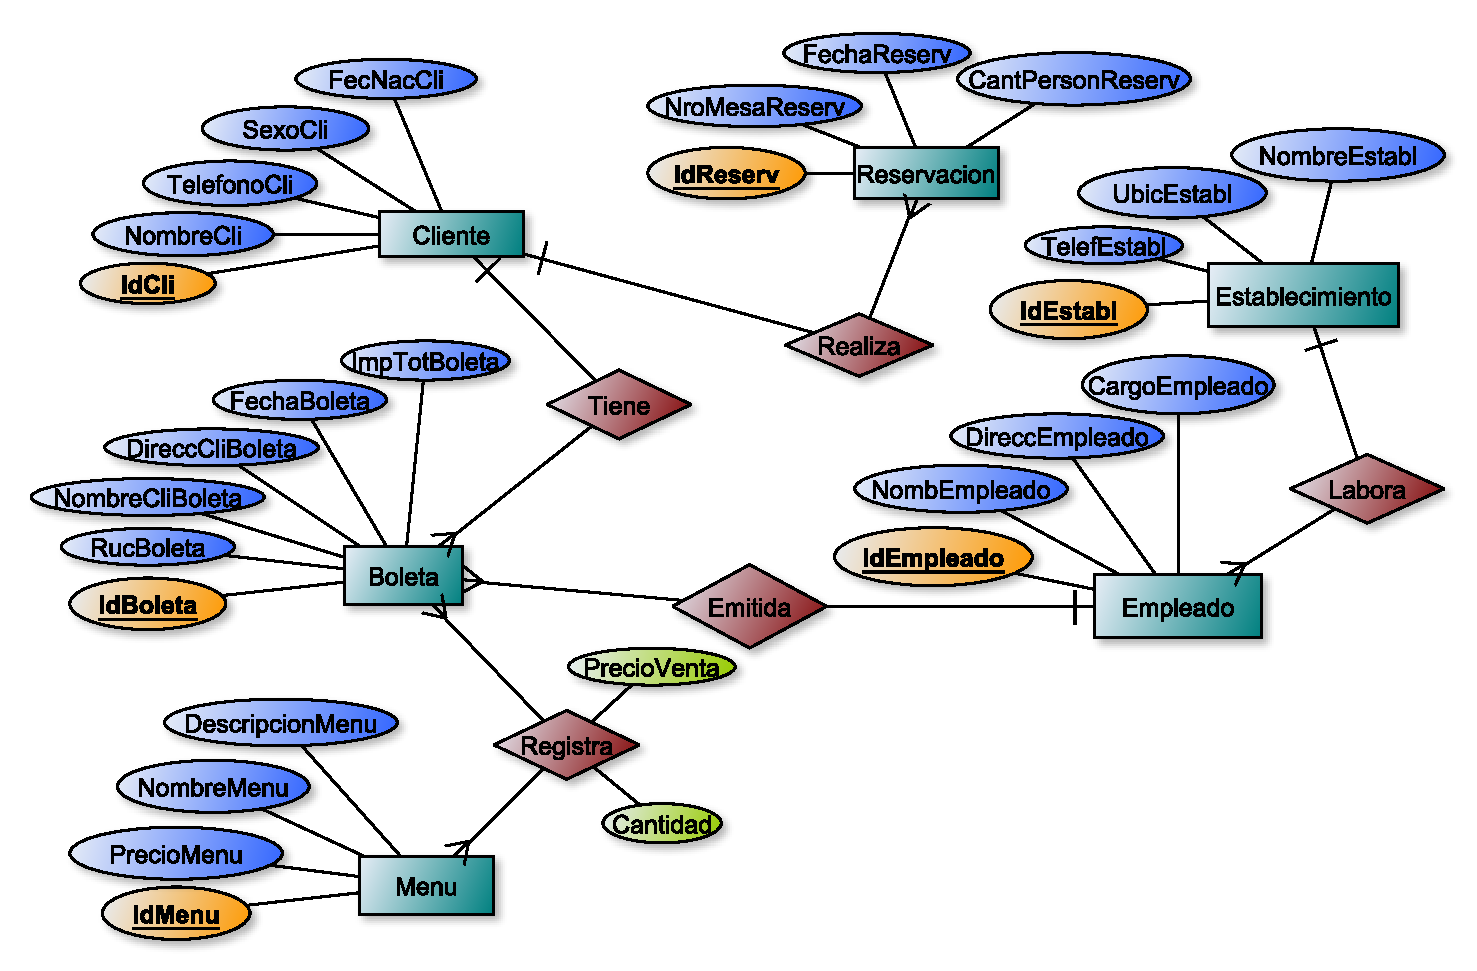
\includegraphics[scale = 0.5]{DER.pdf}
			\caption{Diagrama Entidad Relación}
		\end{figure}
	La lectura es los siguiente (según la regla del negocio): un autor puede tener muchos libros y un libro puede tener muchos autores; un estudiante puede solicitar muchos libros y un libro es solicitado solamente por un estudiante.
	% Pregunta 3
	\section*{Cree una base datos con validación de existencia. Defina su archivo primario y el de registro de transacciones. 1 pto}
	
	A continuación se muestra el código en Microsoft SQL Server Management Studio.
		% Código SQL server
		\lstinputlisting[language=SQL]{SQLQuery1.sql}
	Los códigos previos validan la existencia de la base de datos Bilbioteca y se crea una base de datos con el nombre \textcolor{blue}{BBDD$\_$Biblioteca}
	
	% Pregunta 4
	\section*{Cree las tablas necesarias y sus relaciones para implementar el DER propuesto. 3 ptos}
	
	A continuación se muestra el código en Microsoft SQL Server Management Studio.
		% Código SQL server
		\lstinputlisting[language=SQL]{SQLQuery2.sql}
	Los códigos previos crean las tablas de Autor, Libro, Estudiante y DetalleEstudianteLibro más las relaciones entre ellas.
	% Pregunta 5
	\section*{Ingrese 3 registros en cada tabla. 2 ptos}
	
	A continuación se muestra el código en Microsoft SQL Server Management Studio.
		% Código SQL server
		\lstinputlisting[language=SQL]{SQLQuery3.sql}
	Los códigos previos ingresan 3 registros en cada una de las tablas especificadas.
	% Pregunta 6
	\section*{Cree una consulta usando 1 tabla. Debe considerar en la consulta el uso de alias en los campos, funciones de cadena y de fecha. Especificar condiciones usando operador OR o AND, usar el operador LIKE e IN. Aplicar ordenamiento. Coloque el código T/SQL y 
	adjunte pantalla de resultados. 3 ptos}
	
	A continuación se muestra el código en Microsoft SQL Server Management Studio.
		% Código SQL server
		\lstinputlisting[language=SQL]{SQLQuery4.sql}
	Los códigos previos crean una consulta usando solamente una tabla, considerando los alias, algunas funciones y condiciones.
	
	Asimismo, a continuación adjuntamos la pantalla del resultado:
		% Pantalla de resultados como figura
		\begin{figure}[H]
			\centering
			\includegraphics[scale = 1.5]{Figure1.png}
			\caption{Resultado de la consulta usando 1 tabla}
		\end{figure}
	% Pregunta 7
	\section*{Cree una consulta usando 3 tablas. Debe considerar en la consulta el uso de funciones de cadena y de fecha. Especificar condiciones usando operador OR o AND y aplicar ordenamiento. Coloque el código T/SQL y adjunte pantalla de resultados. 4 ptos}
	
	A continuación se muestra el código en Microsoft SQL Server Management Studio.
		% Código SQL server
		\lstinputlisting[language=SQL]{SQLQuery5.sql}
	Los códigos previos crean una consulta usando 3 tablas, considerando funciones y condiciones ordenados de manera ascendente.
		% Pantalla de resultados como figura
		\begin{figure}[H]
			\centering
			\includegraphics[scale = 0.87]{Figure2.png}
			\caption{Resultado de la consulta usando 3 tabla}
		\end{figure}
	% Pregunta 8
	\section*{Cree un SP con un parámetro, usar 2 tablas y considerar el operador BETWEEN. Invoque el sp con parámetro de ejemplo. Debe salir un registro resultante por lo menos. Coloque el código T/SQL y adjunte pantalla de resultados. 5 ptos}
	
	A continuación se muestra el código en Microsoft SQL Server Management Studio.
		% Código SQL server
		\lstinputlisting[language=SQL]{SQLQuery6.sql}
	Los códigos previos crean un procedimiento almacenado con un parámetro usando dos tablas, considerando el operador BETWEEN y ejecutando el procedimiento almacenado con un parámetro.
		% Pantalla de resultados como figura
		\begin{figure}[H]
			\centering
			\includegraphics[scale = 1.2]{Figure3.png}
			\caption{Resultado del Procedimiento Almacenado}
		\end{figure}
\end{document}



